\section{Configurazione dell'ambiente di lavoro}
\subsection{Configurazione ambiente di sviluppo integrato WebStorm}
La configurazione base di WebStorm prevede la corretta configurazione dei path di sistema\glosp e l'apertura di un progetto.
\subsubsection{Configurazione dei path di sistema}
Aprire le impostazioni di WebStorm dal suo menù "File" ed utilizzando la barra di ricerca cercare "Node.js and NPM". Verificare quindi che entrambe le voci "Node interpreter" e "Package manager" siano correttamente impostate.
\\
\\
\begin{figure}[H] 	
	\begin{center}
		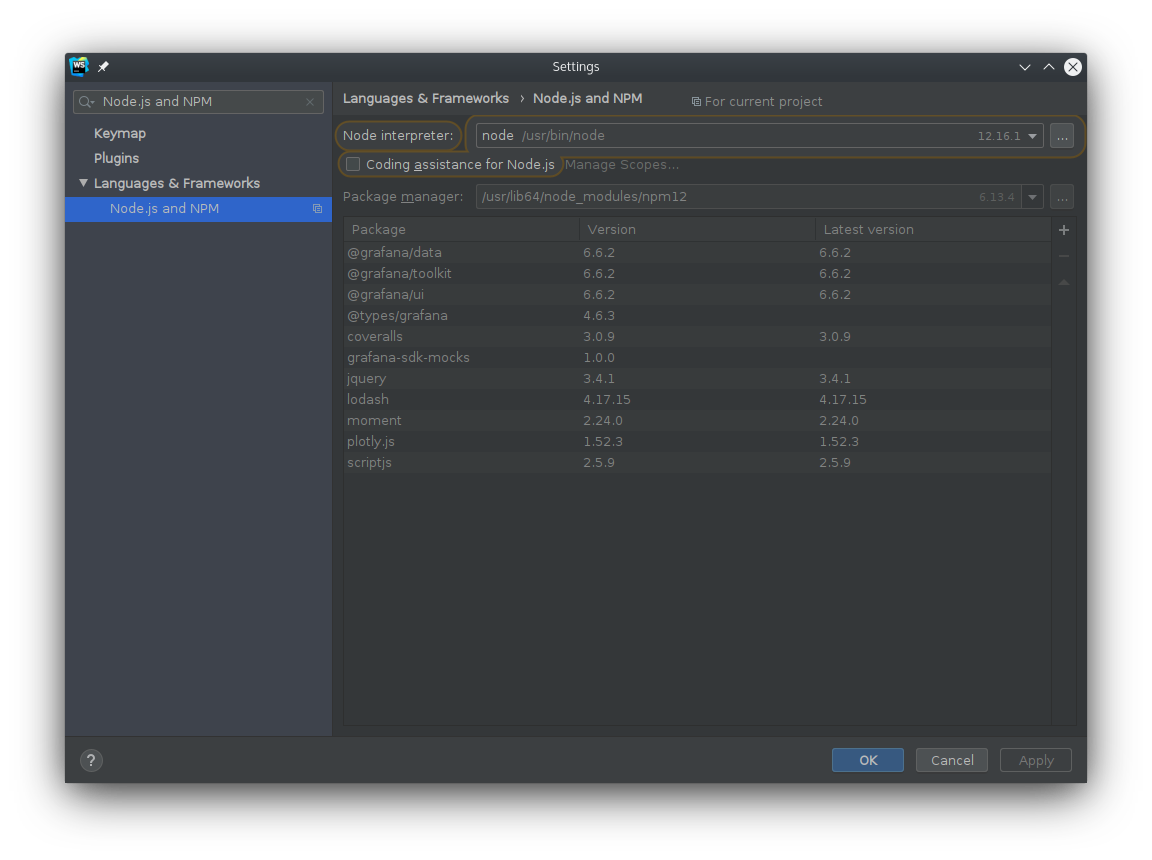
\includegraphics[width=\textwidth,height=\textheight,keepaspectratio]{img/node-npm.png}
	\end{center}
	\caption{Configurazione path di sistema}	
\end{figure}
\subsubsection{Importazione di un progetto}
Dal menu "File" selezionare la voce "Open" e successivamente la root directory del repository desiderato.

\subsection{Configurazione plug-in SonarLint per WebStorm}
\subsubsection{Configurazione globale}
Per configurare il plug-in SonarLint, aprire le impostazioni di WebStorm dal suo menù "File". Quindi nella sezione "Tools" selezionare la voce "SonarLint". Nella finestra "Visualizzare", selezionare il "+" per aggiungere una connessione al servizio WEB SonarCloud.
\\
\\
\begin{figure}[H] 	
	\begin{center}
		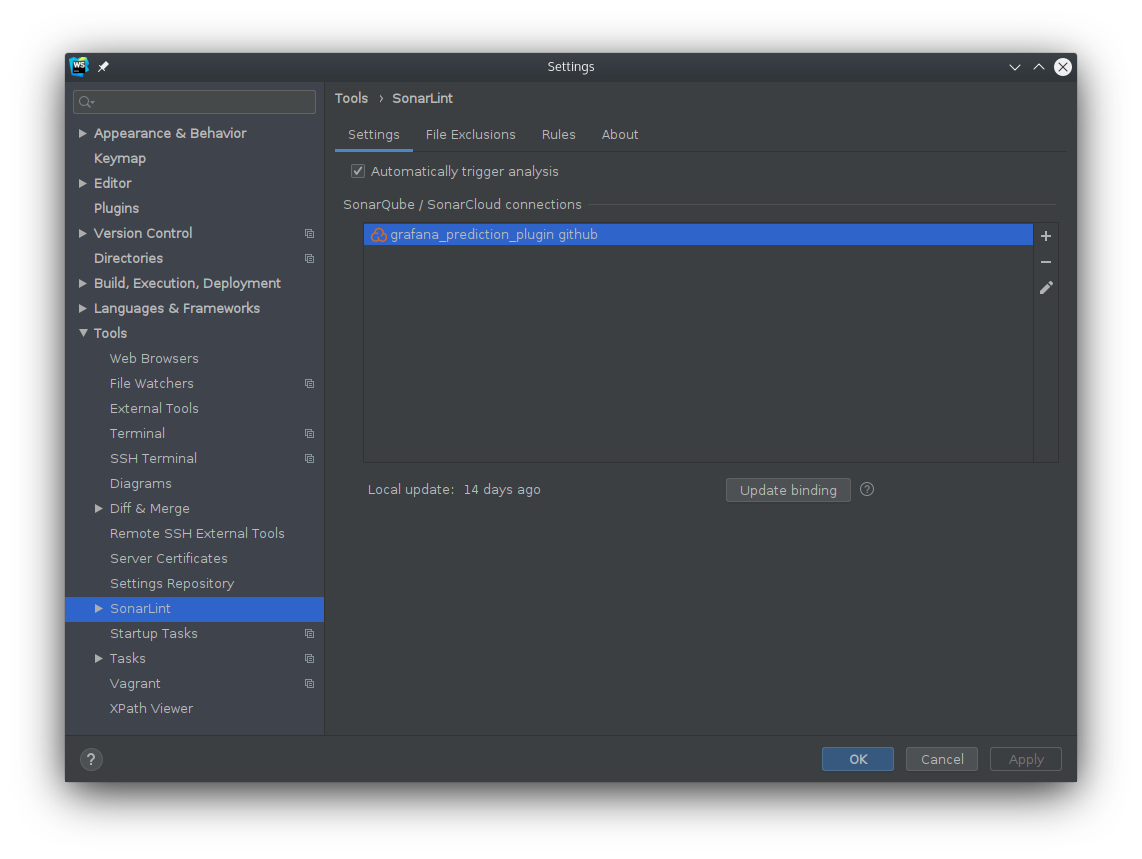
\includegraphics[width=\textwidth,height=\textheight,keepaspectratio]{img/connection.png}
	\end{center}
	\caption{Aggiungere una connessione a SonarCloud}	
\end{figure}
\pagebreak
Dare un nome al collegamento e selezionare SonarCloud, successivamente premere "Next".
\\
\\
\begin{figure}[H] 	
	\begin{center}
		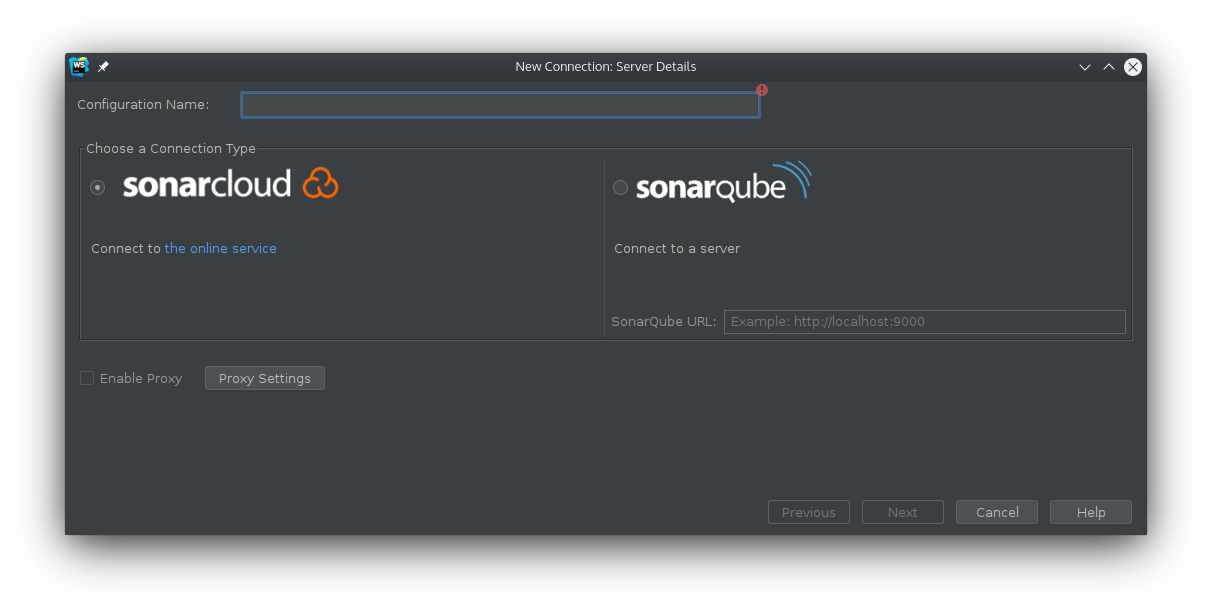
\includegraphics[width=\textwidth,height=\textheight,keepaspectratio]{img/connection-name.png}
	\end{center}
	\caption{Selezionare come collegamento SonarCloud}	
\end{figure}
Premere su "Create Token". Scegliere un nome e creare il token, copiarlo quindi nella finestra WebStorm precedente. \\
%\\
%\\
%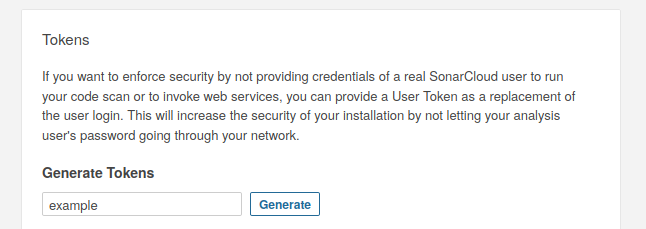
\includegraphics[width=\textwidth,height=\textheight,keepaspectratio]{img/sonarcloud.png}
La connessione viene verificata ed è possibile visualizzarla nell'elenco delle connessioni.
\subsubsection{Configurazione per progetto}
Dopo aver terminato la configurazione globale è possibile configurare i singoli progetti. Per farlo, aprire le impostazioni di WebStorm dal suo menù "File". Quindi, nella sezione "Tools", espandere la voce "SonarLint" e selezionare "Project Settings".
\\
\\
\begin{figure}[H] 	
	\begin{center}
		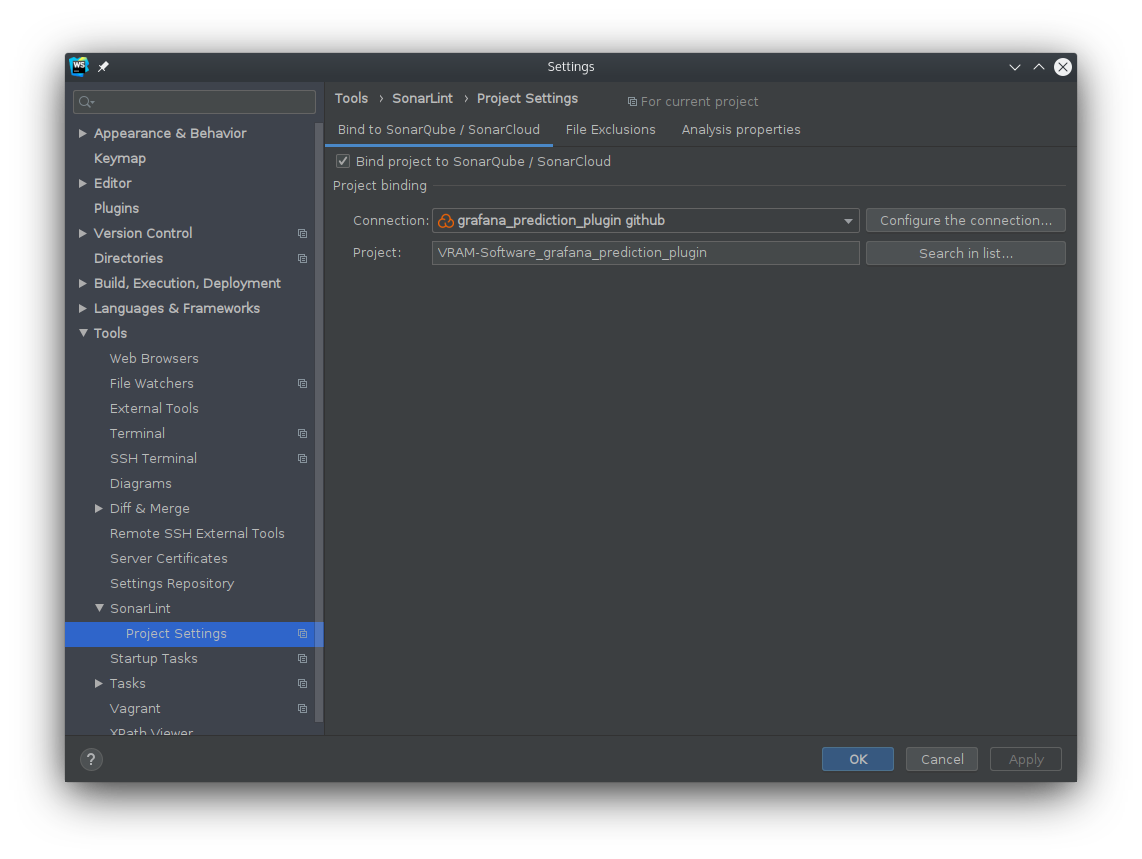
\includegraphics[width=\textwidth,height=\textheight,keepaspectratio]{img/sonarlint-project.png}
	\end{center}
	\caption{Impostazione connessione SonarCloud}
\end{figure}

Selezionare la connessione a SonarCloud desiderata ed inserire una delle chiavi seguenti, a seconda del progetto che si sta configurando:
\begin{itemize}
	\item \textbf{plug-in Grafana}: VRAM-Software\_grafana\_prediction\_plugin;
	\item \textbf{Applicativo esterno}: VRAM-Software\_prediction\_configuration\_utility.
\end{itemize}

\subsection{Configurazione ambiente plug-in Grafana}
\subsubsection{Contenuto file package.json}
Il file package.json contiene tutte le informazioni e i requisiti necessari della nostra applicazione. Le informazioni importanti sono i seguenti attributi:
\begin{itemize}
	\item dependencies: contiene la seguente lista di pacchetti che sono necessari per il corretto funzionamento dell'applicazione:
		\begin{itemize}
			\item jquery;
			\item lodash;
			\item plotly.js;
			\item scriptjs;
			\item influx;
			\item luxon;
			\item ml-modules;
			\item rxjs.
		\end{itemize}
	\item devDependencies: questo attributo contiene la seguente lista di pacchetti che sono necessari per il corretto funzionamento dell'applicazione durante lo sviluppo:
		\begin{itemize}
			\item @grafana/data;
			\item @grafana/toolkit;
			\item @grafana/ui;
			\item @types/grafana;
			\item @types/luxon;
			\item grafana-sdk-mocks;
			\item coveralls.
		\end{itemize}
	\item{scripts}: questo attributo contiene una lista di tutti i comandi, utili per uno sviluppatore, che possono essere eseguiti da linea di comando:
		\begin{itemize}
			\item \textbf{build}: il comando seguente genera una cartella chiamata dist che contiene i file di produzione del plug-in Grafana\glo;
			\begin{verbatim}
				npm run build
			\end{verbatim}
			\item \textbf{test}: il comando fa eseguire tutti i test automatici dell'applicazione;
			\begin{verbatim}
				npm run test
			\end{verbatim}
			\item \textbf{dev}: il comando genera una release di debug\glosp da utilizzare durante lo sviluppo, eseguendo inoltre i linting integrati nella dipendenza npm @grafana/toolkit. Non esegue i test automatici;
			\begin{verbatim}
				npm run dev
			\end{verbatim}
			\item \textbf{ci-test}: il comando, pensato per essere eseguito nell'ambiente di continuous integration, fa eseguire tutti i test automatici dell'applicazione e calcola il code coverage del codice;
			\begin{verbatim}
				npm run ci-test
			\end{verbatim}
			\item \textbf{watch}: il comando esegue il comando "dev" in modalità "watch", ovvero segnalando in automatico gli errori di linting durante la scrittura del codice.
			\begin{verbatim}
				npm run watch
			\end{verbatim}
		\end{itemize}
\end{itemize}
